\documentclass[a4paper, 11pt]{article}
% ----- Loading the Package MCMthesis -----
% -----           v 5.01-L            -----
% `tcn' is short for `Team Control Number'.
% You should fill your tcn after the equal sign following tcn.
% The option `sheet' contorls weather the summary sheet
% will appear.
% The option `abstract' controls weather the abstract 
% will appear in the title-page.
\usepackage[tcn = 80370, sheet = true, abstract = false]{MCMthesis}

% ----- Question Mark -----
\problem{C}
% ----- Fonts settings -----
% You may need to install the font files, if it's needed.
% Disable it, if you don't want this font.
\usepackage{palatino}
\usepackage{indentfirst}
% ----- Set the skip betweent the paragraphics -----
\setlength\parskip{.5\baselineskip}
% ----- The name of Abstract ------
\providecommand{\abstractname}{\relax} % <-- Do not modify here.
\renewcommand{\abstractname}{Abstract} % <-- Modify here, if needed*.


% -----------------------------------
% ===== The Title of Your Paper =====
% -----------------------------------
\title{The Research of Energy Profile in southernwest America}
% ---------------------------------------
% ===== The Author(s) of Your Paper =====
% ---------------------------------------
\author{Team 80370}
% ----------------
% ===== Time =====
% ----------------
\date{February 12, 2018}
\begin{document}
% Abstract should be put before `\maketitle'
\begin{abstract}
In this article, we aim to evaluate the development of energy of four states (Arizona, California, New Mexico and Texas) and set goals for the future development through data analysis and modeling.


Firstly, we consider five aspects (the source of the energy consumption and its proportion, output and the proportion of renewable and clean energy , end usage composition and proportion, energy prices and the total energy consumption, population and energy consumption per capita), the related data processing, in the form of, to describe the energy profile of each state. Based on the ordinary least square method, we found Tendency Description Model and analyze the trend of the energy development. We also interpret the result in the following aspects: population, economy, climate, energy policy.


Secondly, after considering several factors which are the most important in the energy profiles, we implement the AHP method to weight these factors and then apply the TOPSIS method to evaluating the energy profiles of the four states. We conclude that in 2009, Arizona has the "best" energy profile.


Then, on the basis of the energy profiles, considering that some other factors (such as the natural environment, population, climate ) that also affect the energy profiles, we select 7 other index to make the profile more complete. We take 5 years as a forecast period, and found the ARIMA model and the Tendency Extrapolation method to forecast the value of the 7 index, so that we can describe the development of energy profiles in 2025 and 2050..


Finally, by using the standard of the evaluation model, combining the criteria of the "best" profile with the forecast data in 2025 and 2050, we set a goal that four states in 2025 and 2025 of clean and renewable energy of four states accounted for 33\% of the proportion of total energy, respectively, of 39\%.Then we started with funding, technology and energy use, combined with the realities of the four states, and proposed four actions that might be taken to achieve the goal.

\begin{keywords}
keyword1; keyword2
\end{keywords}
\end{abstract}
\maketitle
\pagestyle{empty}
\newpage
 %Generate the Table of Contents, if it's needed.
\tableofcontents
\newpage
\pagestyle{fancy}
% The body of your paper


%======================问题介绍====================================
\section{Introduction}







As is universally acknowledged, energy production plays a significant role in the economic activities, industrial production and many other aspects. Therefore, all countries and areas are supposed to apply the most appropriate methods to producing and using energy. Decision makers will definitely carry out a series of measures and policies to cope with energy issues. Governors in different states make compact to cooperate on energy production. As a result, a set of evaluation criteria and standard should be founded to evaluate the performance of energy sectors, and give an appropriate solution to it.



















\section{The Energy Profile of 2009}
\subsection{The Constitution of Energy Profile }
As far as the profile is concerned, we analyze the structure of energy first, which includes the component of energy, end-usage and price. Then we find out that nuclear energy and renewable energy account for rather small portion, so we further analyze the component and the propotion of nuclear energy and renewable energy.


Wood and waste takes rather small proportion of renewable energy, and it has little space for development in terms of practical efficiency. Therefore, although they belong to biomass, we do not take them into account.


Aiming to create a energy profile for each of the four states, we  will demonstrate the energy profile in the following five aspects:

\begin{itemize}
\item Aspect\,1 \,Source of energy consumption and proportion
\item Aspect\,2 \,Consumption of nuclear energy and renewable energy and proportion
\item Aspect\,3 \,Component of the usage of energy and  proportion
\item Aspect\,4 \,Price of energy
\item Aspect\,5\,Total energy consumption, population, and energy consumption per capita
\end{itemize}

According to the attached data file ,we can conclude that:


1.Total energy is composed by clean energy, coal, natural gas and other fossil fuel. 


2.Clean energy includes renewable energy and nuclear energy.


3.Energy are used by industrial sector, residential sector, transportation sector, and commercial sector.
Therefore,through statistical analysis, we can know the data of the index and their corresponding proportion. 


4.In terms of the prices, due to the adjacent position and similar national policies,  the differences of prices are not obvious. Hence, it is rather difficult for us to characterize the energy profile of the four states by figures depicting original data. This is the reason why we carry out the differential processing of data for further analysis. 


5.Total energy consumption, population, and energy consumption per capita has been given.


\subsubsection{Differential processing of energy price}
\begin{itemize}
\item Step 1:Calculate the average of the corresponding energy price of the four states in identical year. 
$$A=\frac{D_1+D_2+D_3+D_4}{4}$$
where $A $ is the average, $D_i$ is the price of each state.


\item Step 2: Calculate the distance $d_i$ between the price of each state and the average $A $. 
$$d_i=D_i-A$$

\item Step 3: Make the distance $d_i$ dimentionless, and use the percentage $p_i$ as the measurement, where: 
$$p_i=\frac{100\cdot d_i}{A}$$


\end{itemize}














\newpage
\subsection{The Energy Profile }
\subsubsection{The Energy Profile of Arizona}


\begin{figure}[h]

\centering
\includegraphics[width=15cm]{AZ.eps}
\caption{The Energy Profile of Arizona} \label{fig:aa}
\end{figure}
\small
Arizona has a population of 6.587 million and  consume 1,400,000 billion Btu energy in total, which means the consumption per capita is 0.221 billion Btu.


The energy profile of Arizona indicates that nuclear energy has the largest proportion of total energy. The amount of the nuclear energy consumption is nearly the same as the consumption of motor gasoline. 


The transportation sector consume over 50\% of the total energy, while the industrial sector .


Apparantly, in terms of  the renewable energy of Arizona, the consumption of nuclear energy takes the largest portion of 79\%, which  is followed by hydroelectricity(15\%), while that of geothermal energy, wind energy, biomass ethanol along with photovoltaic energy  takes merely 6\% of the total consumption.


When it comes to the price of energy, the price of natural gas in Arizona is far higher than those in the rest three states,  while the price of coal is much lower than the average. Except for the petroleum price in the electric power sector, the petroleum prices in other sectors are almost the same as that in other three states.








\newpage
\subsubsection{The Energy Profile of California}

\begin{figure}[h]

\centering
\includegraphics[width=15cm]{CA.eps}
\caption{The Energy Profile of California} \label{fig:aa}
\end{figure}


California has a population of 36.887 million and  consume 8,000,000 billion Btu energy in total, which means the consumption per capita is 0.217 billion Btu. 


The component of renewable energy is diversified, with the proportion of nuclear energy reaching 37\%, the water energy is 31\%, the geothermal energy is 14c, the biomass is 9c, and the remaining 7c is wind energy and photovoltaic energy. 


In terms of the usage of energy in California, the industrial sector consumed less energy than that in other three states. Half of the energy is used for transportation

In California, coal's heat (2,403 billion Btu) accounts for just 0.67 percent of all energy  (7,805,499 billion Btu), which is different from the other three states. Nuclear and renewable energy accounted for 13 percent of the total, which is the highest among the four states. Natural gas and gasoline are the major energy sources in California. 


California's electricity and coal prices are higher than the average of four states;Household and commercial gas are below the average of 15c to 20c, while industrial and transport prices are above the average of 30 to 40c.Among them,  petroleum products average price in the electric power sector (PAEID) is 80c below the average of the four states.


\newpage
\subsubsection{The Energy Profile of New Mexico}

\begin{figure}[h]

\centering
\includegraphics[width=15cm]{NM.eps}
\caption{The Energy Profile of New Mexico} \label{fig:aa}
\end{figure}

New Mexico has a total energy consumption of about 670,000 billion Btu, with a population of 2,007,000 and consumption per capita of 0.338 billion Btu.


 New Mexico is dominated by coal, petroleum and natural gas (79 percent), and clean energy accounts for 4 percent of the state's energy. 
 
 
 Three-quarters of new Mexico's energy is used for transportation and industry, and a quarter for residential and commercial use.
 
 
  New Mexico has large wind energy source, accounting for nearly 70c of the state's clean energy, followed by biomass energy, hydropower (14c).However, New Mexico do not produce nuclear energy .
 
 
 Except for the electric power sector, prices for all other major energy sources in other sectors are lower or flat than in other states.

\newpage
\subsubsection{The Energy Profile of Texas}

\begin{figure}[h]

\centering
\includegraphics[width=15cm]{TX.eps}
\caption{The Energy Profile of Texas} \label{fig:aa}
\end{figure}
Texas has a total energy consumption is of 12,300,000 billion Btu, with a population of 2,007,000 and consumption per capita of 0.456 billion Btu. 


The main sources of energy are natural gas (1/3), coal (1/6), oil (1/6) and clean energy (6c). 


Industrial sector and transportation sector consume nearly 90 percent of the energy, half of which is consumed by industrial sector. 


Nuclear and wind energy account for 98c clean energy, and the ratio of nuclear energy to wind energy is 3:7. 


Except for the coal price in the industrial sector (CLOCD, CLICD),  electricity, soal, oil, natural gas prices in Texas are lower than or equal to the average of the four states.


\newpage

\section{Energy profile's evolvement from 1960 to 2009}

\subsection{Analysis of the problem}

In order to characterize how the energy profile of each of the four states has evolved from 1960-2009 the four states' usage of cleaner, renewable energy sources, we need to filter the variables for the energy profile. In order to understand the trend clearly, we  need to found a trend model.



\subsection{Tendency description model}

In order to describe the change trend, it is obvious to use the year as the x value, and the data ordinate of the trend description is y value.Since the data is discrete and the data changes are noisy, it is necessary to process the data to describe the trend changes from 1960 to 2009.

\textbf{The implementation of Tendency description model requires the following step:}
\begin{itemize}
\item Step 1:Using the ordinary least square(OLS) method to carry out gaussian curve fitting, Fourier curve fitting and polynomial fitting, to make the discrete data continuous, get fit function $f(x)$.
\item Step 2:Take the derivative of the fitting function, get $f'(x)$, and then find the value of $m$ in the function of the derivative in the year interval.

\item Step 3:The x-range of $|f'(x)|>|m|$ is the change interval of the data, the value of G is the trend of change, '+' is the growth, '-' is decreasing, and the magnitude of the value represents the strength of the trend, and 0 is the same.See the formula:
 $$ G=\left\{
\begin{aligned}
&f'(x), &|f'(x)|>|m| \\
&0, &|m|\leq|f'(x)|\leq|m| \\
 &f'(x), &|f'(x)|<|m| 
 \end{aligned}
\right.
$$
\end{itemize}

\textbf{Strength and weakness}

Strength:This method can be used to infer the direction and intensity of the change trend of the data. By using the value in the function, some fluctuations are reduced.


Weakness:It is not suitable for the data with large fluctuation and long-term fluctuation, which is too large for the trend variation of this kind of model.

\subsection{Tendency description of energy profile}
\begin{itemize}
\item \textbf{Aspect\,1 \,Source of energy consumption and proportion}


We only need to analyze the total energy consumption and clean energy (nuclear power and renewable energy)  by using trend description model. There is no need to analyze coal, oil, natural gas and other non-renewable energy consumption, since it equals to total energy consumption minus the consumption of clean, renewable energy.


\textbf{Tendency description of energy profile} 


See Aspect 5, the trend analysis of Total energy consumption.

\textbf{Electricity produced from nuclear power(NUEGB)} 

\begin{figure}[h]

\centering
\includegraphics[width=15cm]{0.eps}

\end{figure}


All three states have nuclear power and are on the same order of magnitude.California was the first to develop nuclear energy, followed by Arizona, and finally Texas, Texas, which came to the top after about 2003.Nuclear power measuring increase point mutations, and tends to be stable after mutation, consistent with the actual situation, the establishment of a plant, discharge of nuclear power can increase rapidly, discharge of nuclear power is with the size of the plant is.According to the analysis above, after the sudden change of nuclear power, the amount of nuclear power tends to be stable, that is, no new nuclear power plant is established, and the scale of nuclear power plant remains unchanged.





\textbf{Tendency description of  renewable energy production.(REPRB) } 


See Aspect 2, the trend analysis of  renewable  energy production.




\item \textbf{Aspect\,2 \,Consumption of  nuclear energy and renewable energy and proportion}


\textbf{Tendency description of renewable energy production.(REPRB) } 

\begin{figure}[h]

\centering
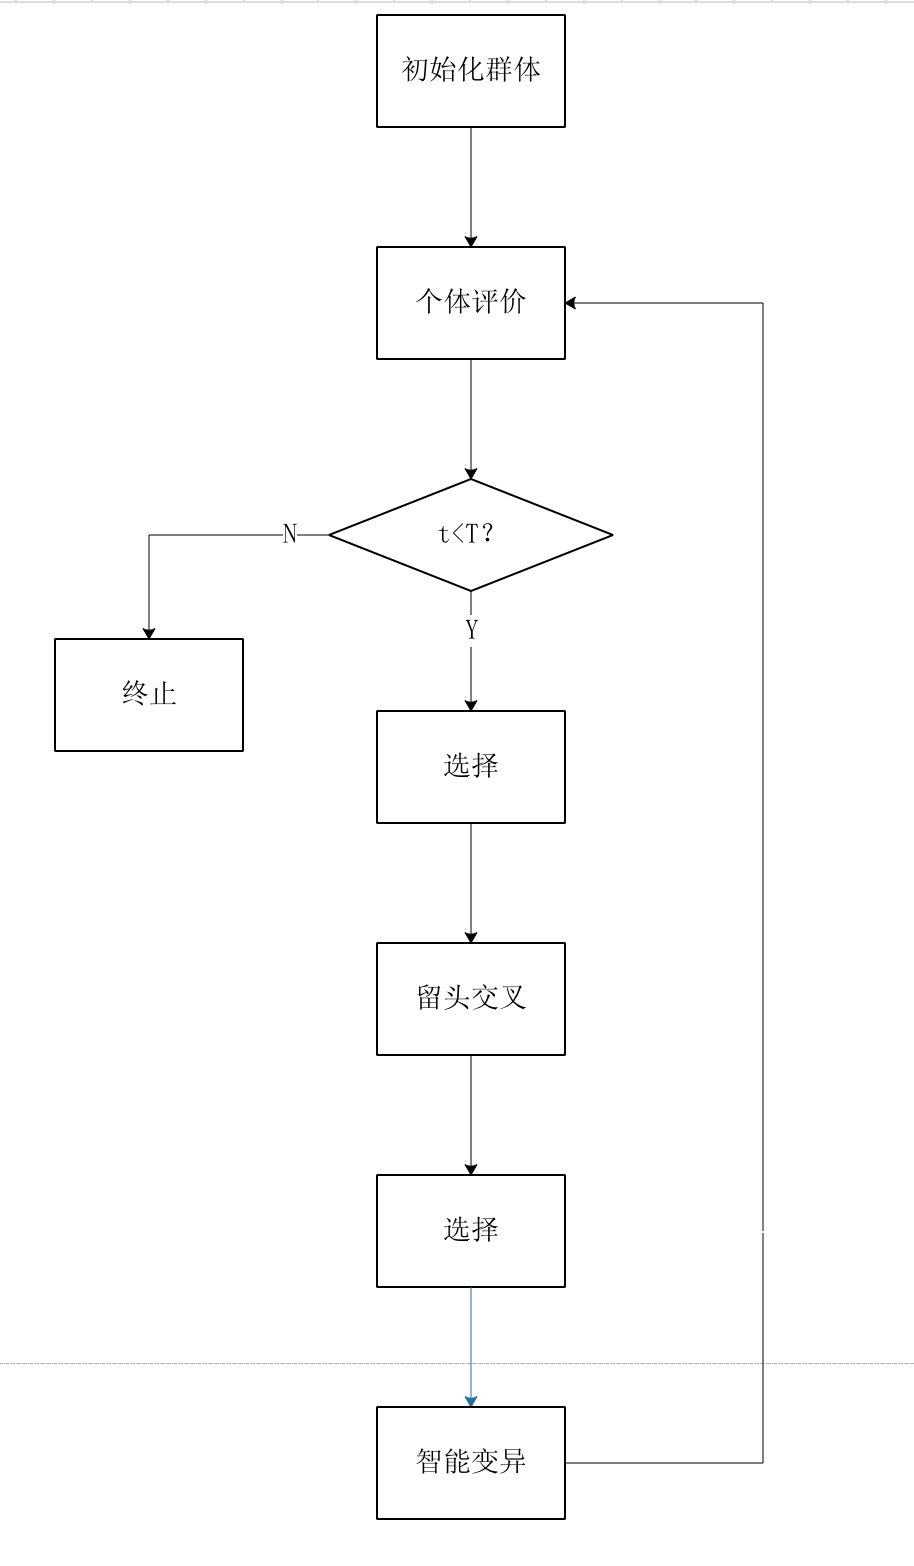
\includegraphics[width=15cm]{2.eps}

\end{figure}



Among the four states, the renewable energy production of Arizona, New Mexico Texas is almost the same, while California has largest output, about four times the first three, from which we can see that California has the earliest development and the fastest pace of development.The trends in renewable energy in the four states fall into two categories:


 The first category contains Texas and New Mexico, where renewable energy developed slowly and then mutated before 2004. To understand the causes of the mutation, we analyzed the various clean energy sources of Texas and New Mexico and found that the contribution of the mutation came from the new clean energy - wind energy introduced by Texas and New Mexico in 2003. It can be seen that, for the states where Texas, New Mexico and other clean energy sources are relatively single and slow to develop, the introduction of new clean energy. 


 The second category includes Arizona and California. Its renewable energy has long been developed, and its overall trend is increasing. However, the data of renewable energy production fluctuates greatly, and there are periodic fluctuations, which cannot be analyzed by the model. Therefore, we adopt the artificial analysis method.
Take Arizona as an example. Renewable energy production in Arizona increased approximately linearly from 1960 to 1980 and peaked around 1983 with a peak at about twice the previous peak, then a sharp decline after 1985 and a return to 1980 levels in 1990. As a new energy source, the conversion efficiency of renewable energy is not high, resulting in increasing costs of energy production. According to the current issue of the development of renewable energy, the strong fluctuation of renewable energy output in the chart is likely to be related to government funding and the technological level of renewable energy. In the early days, the government provided funds to enable the rapid development of renewable energy, due to variable costs, resulting in increased government funding gap, renewable energy companies have suffered losses or even collapse, and then lead to the fall in the output of renewable energy.



\textbf{Electricity produced from nuclear power(NUEGB)} 



See Aspect 1, the trend analysis of  nuclear power(NUEGB).


\item \textbf{Aspect\,3 \,Component of the usage of energy and  proportion}


According to the previous data, the variation range of component of the usage of energy and proportion was all within 10\%, and the distribution and proportion of energy usage did not change significantly.
\item \textbf{Aspect\,4 \,Price of energy}


Due to the large variable range, and the cumulative effect of inflation year by year, the price of 1960-2009 trends descriptions of energy shows little practical significance, so we eliminated the price trend analysis.
\item \textbf{Aspect\,5\,Total energy consumption, population, and energy consumption per capita}


\textbf{The trend analysis of Total energy consumption per capita.(TETPB)} 
\begin{figure}[h]

\centering
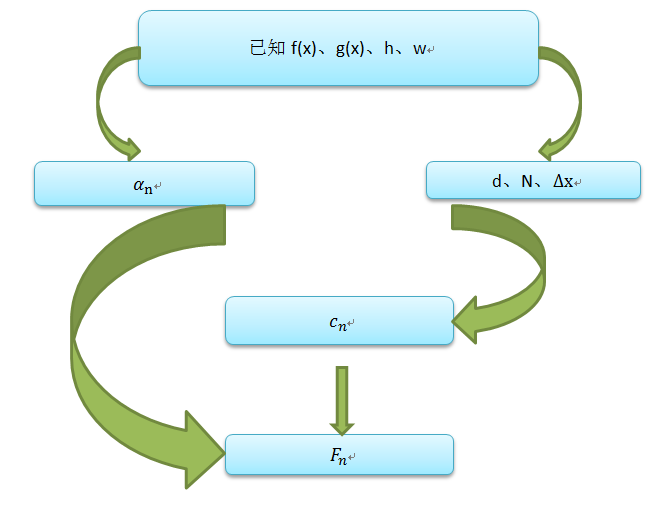
\includegraphics[width=15cm]{1.eps}

\end{figure}



The average energy consumption per capita of the four states peaked between 1973 and 1975, with the annual decrease of Arizona and California after 1975. However, the average energy consumption per capita of New Mexico and Texas in 1975 fluctuated slightly, with the overall decline slightly and steadily. The energy consumption per capita of Arizona and California varies little, and the average energy consumption per capita of these two states is the lowest among four states. The average energy consumption of New Mexico is about 1.5 times of that of Arizona and California, while the average energy consumption of Texas is 2 times of that of Arizona and California.


The reason why is probably that the usage of energy is relatively high in industrial sectors, which leads to the increase of the consumption per capita.


\textbf{The trend analysis of Total energy consumption.(TETCB)} 
\begin{figure}[h]

\centering
\includegraphics[width=15cm]{3.eps}

\end{figure}
The overall trend of the four states is on the rise, with the approximate linear growth of 1975, the growth rate of 1975-2007 slowing down, and the decline in 2007-2009. Before 1975, the linear growth of the four states can probably explained by the result of the second industrial revolution, when large amount of energy was required for the economy growth. After 1975, it is probable that the government take  corresponding measures to improve the energy structure so that the consumption of energy slow down.

\end{itemize}
\subsection{Summary for the governors}

\begin{itemize}
\item Total energy consumption has slowed over the past 60 year, and there is even a trend of falling in recent years.
\item Energy consumption per capita  in four states has a downward trend;The energy consumption per capita  of New Mexico is about 1.5 times that of Arizona and California, while Texas is 2 times that of Arizona and California, mainly because the energy of New Mexico and Texas is relatively high in industrial use.
\item The establishment of nuclear power stations can quickly increase the proportion of local clean energy. New Mexico has no nuclear power plant and the governors can consider building nuclear power plants to increase the proportion of local clean energy. The nuclear power development of Arizona, California and Texas is better.
\item Renewable energy could be related to the development of government financial support and the technical level of renewable energy. In full development of the market economy environment, it needs the support of government departments and related technology development;For states with clean energy, such as Texas and New Mexico, the introduction of new clean energy sources can have a significant effect on the development of local clean energy.

\end{itemize}






\newpage
\section{Evaluation of the energy profiles}
\subsection{Determine the weight of index by applying AHP method}
Analysis Hierarchy Process (AHP) is a popular method to decision making, which splits a decision problem into several independent hierarchical levels that analyzed separately. This method can render a more reasonable and convincing evaluation criteria systematically.


An hierarchy may contain the overall objectives, decision criteria and scenarios. Through the judgment of the preference of different criteria, we can acquire the pairwise comparison matrix. Then by calculating the largest eigenvalue and the corresponding eigenvector, we can get the weight vector of the proposed criteria. Last but not least, by examining the consistency of the pairwise matrix, we can test if we have provide with an appropriate comparison. 
\subsubsection{Determination of evaluation index}
In the previous section, energy profiles of the four states have been provided, which has largely decrease the number of variables given in the attached data file. According to the analysis above and consideration of the factors in the following table, we can determine the index we use to evaluate the profiles of the four states.

	
\begin{table}[!htbp]
\centering
\begin{tabular}{|c|c|} %表格7列 全部居中显示
\hline
Category&Factors\\
\hline
\multirow{3}*{Environment}&Development potentiality\\  %纵向合并4行单元格 
\cline{2-2}  %为第二列到第七列添加横线
&Geographical advantages and limitation\\
\cline{2-2}
&Technology Maturity\\

\hline
\multirow{2}*{Economy}&Total expenditure\\  %纵向合并4行单元格 
\cline{2-2}  %为第二列到第七列添加横线
&Devotion to GDP\\

\hline
\multirow{2}*{Environment}&Environmental friendliness\\  %纵向合并4行单元格 
\cline{2-2}  %为第二列到第七列添加横线
&Potential hazards\\

\hline
\end{tabular}
\caption{Significant factors proposed to be considered in the determination}
\end{table}







\begin{figure}[h]

\centering
\includegraphics[width=12cm]{1.c.eps}
\caption{The hierarchy of evaluation index of AHP} \label{fig:The hierarchy of evaluation index of AHP}
\end{figure}



\newpage
\subsubsection{Implementation of AHP}
After weighting the preference of the index according to the factors listing in Table 1 above, now we have the pairwise matrix of the index.


\begin{table}[!htbp]
\center
\begin{tabular}{|c|c|c|c|c|}


\hline
  &1	&2&	3	&Weight\\
\hline

$C_1$&1	&1/3&	5	&0.2790\\
\hline
$C_2$&3	&1	&7	&0.6491\\
\hline
$C_3$&1/5	&1/7	&1&	0.0719\\
\hline
\end{tabular} 
\caption{The pairwise matrix of the index in the second hierarchy}
\end{table}


\begin{table}[!htbp]
\center
\begin{tabular}{|c|c|c|c|c|c|c|c|}


\hline
  &1	&2	&3	&4	&5	&6	&Weight\\
\hline

$C_{11}$&1	&1/3	&1/5	&1/7&	1/5	&1/9	&0.0304\\
\hline
$C_{12}$&3	&1	&1/3&	1/3	&1/3	&1/4	&0.0691\\
\hline
$C_{13}$&5	&3	&1	&1/2&	1/2&	1/2	&0.1418\\
\hline
$C_{14}$&7	&3	&2	&1	&1	&1/3&	0.1948\\
\hline
$C_{15}$&5	&3	&2	&1	&1	&1/3	&0.1851\\
\hline
$C_{16}$&9	&4	&2	&3	&3	&1	&0.3788\\
\hline
\end{tabular} 
\caption{The pairwise matrix of the index in the second hierarchy}
\end{table}

Eventually, we have the weight of all index, which is listed in the following table.


\begin{table}[!htbp]
\center
\begin{tabular}{|c|c|c|c|c|c|c|c|c|}



\hline

Index&$C_11$&$C_12$&$C_13$&$C_14$&$C_15$&$C_16$&$C_2$&$C_3$\\
\hline
Weight&0.0085&	0.0193&	0.0396&	0.0544&	0.0516&	0.1057&	0.6491&	0.0719\\
\hline

\end{tabular} 
\caption{Weight of all index}
\end{table}


\subsection{Determine the "best" profile by applying TOPSIS method}
	TOPSIS is a multi-criteria decision making method that provide us with a ranking of alternatives. It is based on the concept of distance between each alternative and both the positive ideal solution and the negative ideal solution. The "distance" here refer to Euclid distance. Therefore, the best alternative is the nearest to the positive ideal solution, and the farthest from the negative ideal solution. 
 
 
 \textbf{The implementation of TOPSIS requires the following step:}
\begin{itemize} 
 \item Step 1: Solve the normalized decision matrix. While the decision matrix in this problem is  $A = {({a_{ij}})_{m \times n}}$, the corresponding normalized decision matrix is $B = {({b_{ij}})_{m \times n}}$, where
	 $${b_{ij}} = \frac{{{a_{ij}}}}{{\sqrt {\sum\limits_{i = 1}^n {{a_{ij}}^2} } }} , where i = 1,2,...,m, j = 1,2,...,n$$


\item Step 2: Weight the evaluation criteria. In this problem, the weight vector $\omega  = {({w_1},...,{w_n})^T}$has been acquired in the previous section (Table 3). Create the weighted and normalized decision matrix  $C= {({c_{ij}})_{m \times n}}$, where
	 $${c_{ij}} = {w_{ij}} \cdot {b_{ij}} , where ,i = 1,2,...,m j = 1,2,...,n$$


\item Step 3: Identify the positive ideal solution  ${C^*}$ and the negative ideal solution  ,${C^0}$ where
	
 
$${C^*} = ({c_1}^*,...,{c_k}^*) = \left\{ {\begin{array}{*{20}{c}}
{\max {c_{ij}},j \in I'}\\
{\min {c_{ij}},j \in I''}
\end{array}} \right. ,   j = 1,2,...,n$$
	  
$${C^0} = ({c_1}^0,...,{c_k}^0) = \left\{ {\begin{array}{*{20}{c}}
{\min {c_{ij}},j \in I'}\\
{\max {c_{ij}},j \in I''}
\end{array}} \right.,  j = 1,2,...,n$$
   where  $I'$ and  $I''$ are the sets of criteria to be maximized and minimized respectively.

\item Step 4: Calculate the distance between alternatives and both the positive ideal solution and the negative ideal solution. The distance between alternative   and the positive ideal solution is defined as
	  
\[{s_i}^* = \sqrt {\sum\limits_{i = 1}^n {{{({c_{ij}} - {c_j}^*)}^2}} } ,i = 1,2,...,m\]
While the distance between alternative   and the negative ideal solution is defined as
	  
\[{s_i}^0 = \sqrt {\sum\limits_{i = 1}^n {{{({c_{ij}} - {c_j}^0)}^2}} } ,i = 1,2,...,m\]

\item Step 5: Characterize each solution i by the related closeness coefficient  ${f_i}^*$

\item Step 6: Rank the alternatives in the descend order of  .


After programming in Matlab 2016b, we eventually have the related closeness coefficient of the profiles of the four states.


\begin{table}[!htbp]
\center
\begin{tabular}{|c|c|c|c|c|}


\hline
 State&	Arizona&	California&	New Mexico&	Texas\\
\hline

$f_i^*$&0.8659&	0.3447&	0.0905&	0.1892\\
\hline
Rank&	1&	2	&4&	3\\

\hline
\end{tabular} 
\caption{The $f_i^*$ and rank of the four states}
\end{table}


 

\end{itemize}


In conclusion, Arizona has the "best" profile for using clean, renewable energy.

\subsection{Strength and weakness}
Strength
\begin{itemize}
\item	Easy to implement. The mechanism of AHP method TOPSIS method are quite easy to understand, and we can be familiar with the basic steps without difficulties. What's more, the calculation is not complex, but the model can rank the profile in a quite convincing way.
\item	Systematicness. 
\end{itemize}

Weakness
\begin{itemize}
\item Subjectivity. All the comparison in the pairwise comparison matrix is determined by the decision maker.
\item	Roughness. The model cannot include all the factors that may affect the energy profile.
\item	No real optimal scheme. The TOPSIS method merely gives a relative rank of the four states. However, due to the mechanism of this method, it cannot provide with an optimal profile.
\end{itemize}



\section{Energy Profile Index Forecast (EPIF) Model}

In Energy Profile, we initially choose the usage and proportion of each category of energy, the proportion of nuclear energy and renewable energy, and the average price of energy as factors to describe the energy profiles of the four states. In fact, however, some other factors, such as the natural environment, the developing prospect of energy sector, population, local climate, technology, local GDP, can also affect the energy profiles. Therefore, we select the following 7 index to complete the energy profiles so that we are able to describe the difference of the situation of the energy development comprehensively.
  \begin{itemize}
\item Total energy consumption.
\item Primary energy total consumption.
\item Renewable energy total consumption. 
\item Electricity total consumption.
\item Total energy average price.
\item Total energy consumption per capita. 
\item  Energy expenditures as share of current-dollar GDP.

\end{itemize}

Under the circumstance that no policy changes will take place in the future, we can assume that all index of the energy profile will develop in a consistent tendency. Therefore, basing upon we found the ARIMA model combined with tendency extrapolation.
\subsection{Data Processing}
As is universally acknowledged, local energy policies can largely affect the energy profile, but it may take much time to be effective. With this consideration, we assume that there is no change in policy every five year. In order to minimize the effect of some specific events (e.g. the financial crisis in 2008) and shorten the forecast period, we process the data by the following method:

$${x'_i} = \frac{{\sum\limits_{j = 0}^4 {{x_{1960 + 5i - 5 + j}}} }}{5}(i = 1{\rm{,}}2{\rm{,}}3...)$$
\subsection{The Foundation of Model}

\begin{figure}[h]

\centering
\includegraphics[width=12cm]{1d.eps}
\caption{The process of EPIF model} \label{fig:aa}
\end{figure}

After testing of the model, we have the ARIMA model:
 ,
\[{\hat y_i} = \mu  + {\phi _1}*{y_{i - 1}} + ... + {\phi _p}*{y_{i - p}} + {\theta _1}*{\varepsilon _{i - 1}} + ... + {\theta _q}*{\varepsilon _{i - q}}\]

where  $\hat y_i$is the predictive value, $ {y_i}$is the stable series after difference,  .\[{y_i} = {\nabla ^d}{x_i}\]
where :\[\{ {\nabla ^d}{x_i}\} \]
	  
\[{\nabla ^1}{x_i} = {x_i} - {x_{i - 1}}\]
	  
\[{\nabla ^d}{x_i} = {\nabla ^{d - 1}}{x_i} - {\nabla ^{d - 1}}{x_{i - 1}}\]
  $\phi $is the coefficient of AR,   $\theta $is the coefficient of MA, and  $ {\varepsilon _i}$is the error sequence.





 If the pure randomness and the ARIMA model test are not passed, we cannot forecast the data with the ARIMA model. Due to the consistence of the developing tendency, we apply the Tendency Extrapolation method so that we can get an appropriate function to reflect the tendency as well as forecast.


(1)	The selection of model

Now we have the graphs of variables vary according to the timeline. Compare them with the graphs of curves of different kinds of functions so that we can choose a few appropriate models. Through testing the determination coefficient  $R^2$of the sample or the standard error  $SE$,we can choose the most appropriate model. Here:
 
\[{R^2} = \frac{{\sum {{{(\hat y - \bar y)}^2}} }}{{\sum {{{(y - \bar y)}^2}} }} = 1 - \frac{{\sum {{{(y - \hat y)}^2}} }}{{\sum {{{(y - \bar y)}^2}} }}\]
 
\[SE = \sqrt {\frac{{\sum {{{(y - \hat y)}^2}} }}{n}} \]
(2)parameter estimation

For linear models, we can apply Ordinary Least Square method (OLS) to estimate parameters. In addition, OLS can also be applied in models that can be transformed to linear models by taking the inverse or the logarithm of the variables.



For those models which cannot be transformed to linear models, we apply Gauss-Newton Iteration Method to estimate parameters, that is to say, applying Taylor Expansion to the model and then applying iterative methods to estimate.   

\subsection{The solution of model}
According to the forecast model, now we have the predictive index of energy profile of the four states listed in the following table.
Forecast of the energy development situation in 2025 and 2050.
\begin{figure}[h]

\centering
\includegraphics[width=12cm]{chart.eps}
\caption{Forecast of the energy development situation in 2025 and 2050} 
\end{figure}



\newpage
\subsection{Analysis of the result}


Through the longitudinal analysis of data, we can find out the general trend of energy development in each state in the future. Through the horizontal analysis of the data (the comparison of the same index data at the same time in different states), we can make a assessment of the energy developing situation of different states in the future.



Due to the limitation of length, we take the cases of California (California) and Arizona (Arizona) as examples to explain our model results.


1) Longitudinal analysis: For total energy consumption in Arizona (Arizona), compared with 2009, the average annual consumption increases in 2025 and 2050, and the growth is clear. It can be estimated that within a period of time after the 2009, the state's total energy consumption overall rise.


2) Lateral comparison: in California (California), Arizona (Arizona) in 2025, the energy state of each index value, for example, the forecast data shows that California's overall energy consumption capacity is higher than the Arizona, at the same time, the state of California to each kind of energy consumption is relatively more, both the average energy prices, per capita energy consumption, energy spending as a share of GDP.


\section{Goals and action}
\subsection{ Goals of the index of the usage of renewable energy in 2025 and 2050}
In Evaluation of the energy profiles, we found the model of evaluating energy profile of the four states by applying AHP method. Among them, we use 2009, clean and renewable energy use accounted for the ratio of the total amount of energy use and energy use compared to 2008 growth rate as the evaluation index of the first layer, finally draws the conclusion that Arizona has the "best" energy profile. Therefore, we have reason to believe: in the absence of policy adjustment, in 2025 and 2050, clean and renewable energy is still the optimal condition Arizona. In this problem, we use the largest index weight evaluation index Evaluation of the energy profiles of the first layer we use: clean and renewable energy accounted for the ratio of the total amount of energy used to the four state to set the target on the use of renewable energy in 2025 and 2050.


The forecast model can be obtained 
by the state energy index 
established by the 
Energy Profile
Index Forecast
 (EPIF) Model in 2025 and 2050, Arizona clean renewable energy accounted for the proportion of total energy are respectively
 33\%, 39\%. We expect the formation of an energy contract in four states that some actions can be taken on to achieved this value in 2025 and 2050. The goal is set: in four states in 2025 and 2050 of the clean renewable energy accounted for the proportion of total energy are respectively 33\%,39\%.
\subsection{Action taken to achieve the goal}
1) Before we set our targets, initially we analyze the usage of clean and renewable energy (nuclear, wind, hydro, solar, geothermal, biomass (ethanol) in 2009 with the state's energy profiles created in Energy profile in 2009 for with the state's energy profiles created in Energy profile .


Arizona:


Arizona's clean and renewable energy sources account for 28\% of total energy, the highest of the four states. Among them, nuclear energy accounts for 17.71\% of all energy in the state and the local gasoline energy is almost equal. Of all clean and renewable energy sources, nuclear energy accounted for the largest share of 79\%, followed by hydroelectric energy, accounting for 15\%, geothermal energy, wind energy, bio-ethanol and solar energy accounting for only 6\%. From the data, we can conclude that the nuclear power in Arizona is more developed, and there is huge potentiality for the development of geothermal energy, wind energy, bio-ethanol and solar energy.


California:	


Clean and renewable energy accounts for 11\%. of total energy. Energy distribution is more diversified. Nuclear power accounted for the highest, which has reached 37\%. Hydropower accounts for 31\%. Geothermal energy accounts for 14\%, the remaining 18\% for wind energy, solar energy, biomass energy.


New Mexico:


Clean energy, renewable energy accounts for 4\% of the statewide, New Mexico wind power is outstanding, the state clean energy accounts for 67\%, followed by biomass (18\%), hydropower (12\%). Utilization of geothermal energy and solar energy is very low, only 3\%, yet to carry on the development and utilization of nuclear energy.


Texas:


The clean, renewable energy accounted for 6\% of total energy, nuclear energy and wind energy accounted for 89\%, the ratio of nuclear energy to wind energy is 2:1. Biomass energy accounted for 9\%, while the geothermal and photovoltaic energy has not been developed.
From the above analysis, the four states all clean and renewable energy contribution for nuclear power, and geothermal energy, solar energy, biomass energy accounted for very little proportion, so there is a larger space for development.
Through further analysis of the clean and renewable energy data of the four states from 1960 to 2009, we can conclude that solar energy and geothermal energy resources of California are rich, and the exploitation technology is in high level.


\subsubsection{ The establishment of the action scheme}


The main factors restricting the development of clean renewable energy: technology and capital. In order to achieve the goals set, we start from these two aspects, the energy itself, according to the actual situation of four states, has developed the following action plan:


a.Technical exchanges between the states are necessary. The four states have different levels of technology. For example, the wind industry in Texas is the most prosperous. New Mexico has the highest level of solar energy development and application. So they can pass on the technology to other states, bringing the overall skill levels of the four states to tremendous improvement in the shortest timeframe.


b.According to local conditions, make full use of local geographical location and climate advantages, mining resources, to avoid wastage of resources.  For example, all four states are located on the border between the United States and Mexico. They are located in the tropical Pacific Rim. Their geothermal resources are abundant. However, all four states have relatively low levels of development and utilization. This is a waste of energy.  The state of California is dry and sunny in summer, so there is room for improvement in solar energy utilization in the state.


c.All states should formulate a set of reasonable energy allocation plan so that all the states can play their part in avoiding weaknesses and develop more skilled energy sources in their own countries.


d. Develop nuclear energy in New Mexico. New Mexico, the largest contributor to all clean and renewable energies in the four states, has not yet utilized nuclear power. So New Mexico's nuclear power development, backed by the technical support of other states, is an effective means of promoting clean, renewable energy in the four states.


\section{Memo to the group of Governors}
To: The group of Governors


From: Team 80370


Date: February 12, 2018


Subject: The summary of the state profiles, the predictions and the recommended goals


Dear governors of Arizona, California, New Mexico and Texas:


We create energy profiles for states with total energy consumption, energy consumption per capita, nuclear energy consumption, and renewable energy consumption. Through the analysis of the data, we find that the growth of total energy consumption has been slowing down over the past 50 years, and there is even a trend of falling in recent years. The energy consumption per capita of four states reach the peak between 1973 and 1975, and as a whole has a downward trend, New Mexico's energy consumption per capita is about 1.5 times that of Arizona and California while the Texas for Arizona and California 2 times The reason is probably that the usage of energy is relatively high in industrial sectors, which leads to the increase of the consumption per capita. Among the four states, the renewable energy production of Arizona, New Mexico Texas is almost the same, while California has largest output, about four times the first three, from which we can see that California has the earliest development and the fastest pace of development.


On the basis of the energy profile created in the article, we further selected seven indicators such as total energy consumption to create energy profiles for the states and forecast the value of the seven index in 2025 and 2050, Through the analysis of the result, we can find out that: the total energy, primary energy, clean and renewable energy, the total energy consumption of the four states increase. The average price of energy in four states is basically the same; The energy consumption per capita and energy expenditure in 2050 will be slightly lower than in 2025.By using the standard of the evaluation model, combining the criteria of the "best" profile with the forecast data in 2025 and 2050, we set a goal that four states in 2025 and 2025 of clean and renewable energy of four states accounted for 33\% of the proportion of total energy, respectively, of 39\%.



Best,


Team 80370

















\begin{thebibliography}{99}
%\addcontentsline{toc}{section}{References}
\bibitem{1} Lucie Lidinska1 · Josef,Jablonsky,AHP model for performance evaluation of employees in a Czech management consulting company© Springer-Verlag GmbH Germany 2017
Mathematical Society and Addison-Wesley
Publishing Company , 1984-1986.
\bibitem{2}Silvia Carpitella , Antonella Certa , Joaqun Izquierdo , Concetta Manuela La Fata ,k-out-of-n systems: An exact formula for the stationary availability and multi-objective configuration design based on mathematical programming and TOPSIS ,Journal of Computational and Applied Mathematics


\bibitem{3}https://www.eia.gov
\bibitem{4}https://en.wikipedia.org/wiki/Renewable energy
\end{thebibliography}


\end{document}
% ----- End of Document Body ----- 